\chapter{Marco Teórico} \label{chap:marcoteorico}

En el siguiente capitulo se pondrá al alcance del lector las bases teóricas y los conocimientos necesarios para poder entender las diferentes terminologías utilizadas en el trabajo de investigación realizado.

Se tratará de dar un enfoque simplificado de temas como: ¿que es el sensado remoto?, ¿de que hablamos cuando nos referimos a Machine Learning o Deep Learning?, ¿que son las redes neuronales y para que sirven?, entre otras terminologías.

\section{Sensado Remoto}\label{sec:sensadoremoto}

En esta sección desarrollaremos el principal enfoque de este trabajo que son las imágenes satelitales; para esto debemos hablar de la teledetección.

La teledetección o sensado remoto es el proceso que nos permite obtener una imagen de la superficie terrestre de forma remota, es decir sin estar en contacto con ella. Una imagen satelital es una representación de estos datos reflejados por la superficie terrestre que son captadas por un sensor que se encuentran a bordo de un satélite artificial (ver fig \ref{Fig:teledeteccion}).

La teledetección no es mas que la detección de propiedades relevantes del entorno; esta capacidad no es despreciable, nos permite desarrollar aplicaciones practicas con un impacto cada ves mayor \citep{percepcion}. Los datos captados incluyen desde sensores hiperespectrales, multiespectrales, radares, infrarrojos y ópticos.

\begin{center} \begin{minipage}{0.8\linewidth}  \vspace{5pt} {\small
Either to supplement the capability of sensors or to effectively utilize the enormous amount of sensor data, many advances in statistical pattern recognition can be very useful in machine recognition of the data. The potentials and opportunities of using statistical pattern recognition in remote sensing are indeed unlimited.}
\begin{flushright} (\citeauthor{Ledda})
\end{flushright}
\end{minipage}
\end{center}

\begin{figure}[H] \centering
  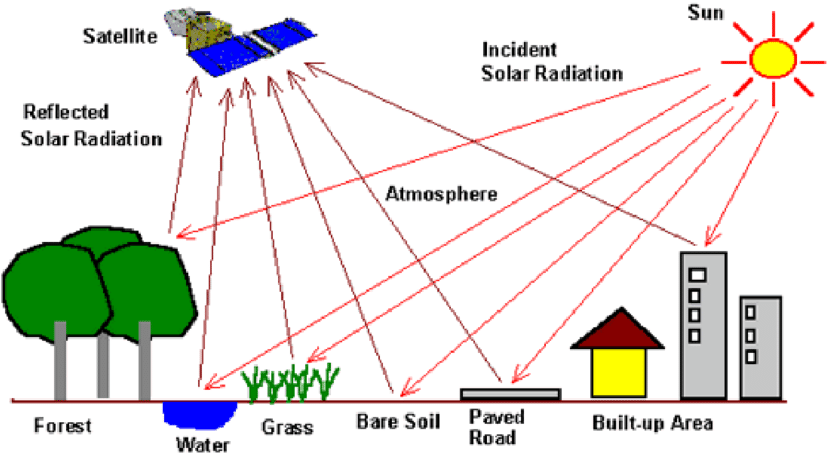
\includegraphics[height=8cm,keepaspectratio=true,clip=true]{imagenes/MarcoTeorico/teledeteccion.png}
  \caption{Sensado Remoto. Navarrete, Edison, Laubacher, Gerard}\label{Fig:teledeteccion}
\end{figure}

Esta disciplina es una las áreas de mayor interés y crecimiento de los últimos años dentro de la informática en el procesamiento de imágenes. La clasificación de imágenes es una de las mayores tareas a la hora de realizar el procesamiento de  las imágenes satelitales y es donde vamos a poner nuestro mayor esfuerzo.

\section{Inteligencia Artificial}\label{sec:inteligenciaA}

En la literatura existe diferentes puntos de vista sobre que es la \ac{ia}, los enfoques que podemos encontrar son aquellos que se refieren a los procesos mentales, razonamiento y la conducta; es decir sistemas: que piensan como humanos, que piensan racionalmente y que actúan como humano \citep{inteligenciaA}. 
\begin{center}
\begin{minipage}{0.8\linewidth}  \vspace{5pt}{\small La \ac{ia} es la parte de la ciencia de la computación que se ocupa del diseño de sistemas computacionales inteligente, es decir, sistemas que exhiben las características que asociamos en el comportamiento humano.}
\begin{flushright}
  ({Barr and Feigembaum})
\end{flushright}
\vspace{5pt}
\end{minipage}
\end{center}

Hay dos corrientes fundamentales  que persiguen los trabajos realizado en \ac{ia}; estos enfoques dependen de diferentes técnicas usadas para la realización de tareas inteligentes. Por un lado un enfoque que apoya a desarrollar programas que reflejen comportamiento de la forma mas eficiente, en esta corriente están las redes neuronales y algoritmo genéticos y por otro lado el que busca los resultados siguiendo procesos cognitivos que realizan las personas \citep{inteligenciaACasali}. La capacidad de aprender es una de las características fundamentales de la inteligencia. 

Partiendo de estas corrientes podemos empezar a desarrollar el papel que juega la \ac{ia} en el campo del procesamiento de imágenes. Existen diferentes ramas dentro de la \ac{ia} que se solapan a la hora de trabajar con procesamiento de imágenes, en la siguiente figura se detallan las mismas (Ver.Fig: \ref{Fig: inteligenciartificial}).

\begin{figure}[h]
 \centering
  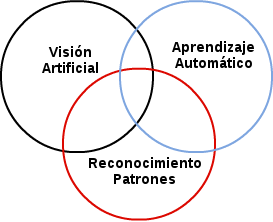
\includegraphics[height=8cm,keepaspectratio=true,clip=true]{imagenes/Logos/va_.png}
  \caption{Ramas de la \ac{ia} y sus relaciones.}
	\label{Fig: inteligenciartificial}
\end{figure}


\section{Visión Artificial}\label{sec:visionartificial}
Como se mostró en la sección anterior (ver: \ref{Fig: inteligenciartificial}), \ac{va} es una rama de la \ac{ia}, que tiene como objetivo extraer información del mundo físico a partir de imágenes, utilizando para esto un procesamiento computacional.

\begin{center}
\begin{minipage}{0.7\linewidth}  \vspace{5pt}{\small La visión por computadora tiene como objetivo el uso de cámaras para analizar o entender escenas en el mundo real.}
\begin{flushright}
  \citep{Reinhard}
\end{flushright}
\vspace{5pt}
\end{minipage}
\end{center}

Esta disciplina estudia problemas metodológicos y algorítmicos como así también temas relacionados con la implementación y diseño de soluciones. En los años recientes la \ac{va} se convirtió en una tecnología clave en muchos campos debido al gran avance en cámara y en procesamiento computacional.

Un sistema de \ac{va} actúa sobre una representación de una realidad que le proporciona información sobre brillo colores, formas, etcétera. Estas representaciones suelen estar en forma de imágenes estáticas, escenas tridimensionales o imágenes en movimiento \citep{Ledda}. 

En \ac{va} tratamos de describir el mundo real que vemos en una o mas imágenes y reconstruir sus propiedades, tal como la forma, iluminación y distribución del color \citep{Szeliski}; con esta disciplina podemos saber en que carril se encuentra un vehículo, cuantas personas hay en una escena, reconocer a una persona en particular; así como lo mencionado, existen numerosas aplicaciones que hoy en día están en el mercado  y usan técnicas de \ac{va}. 

Los campos de aplicación que hacen uso de \ac{va} en diferentes áreas de la ciencia y el mercado son \citep{areascv} :
\begin{enumerate}
\item Robótica : Se usan técnicas de \ac{va} con el fin de reconstruir la escena e identificar los objetos.
\item Biología : En el campo de la biología podríamos distinguir entre aplicaciones microscópicas y macroscópicas. En una imagen microscópica  podemos  usar técnicas de segmentación para contar el número de microorganismos o células presentes en la imagen.
\item Medicina : Para este campo existen muchas aplicaciones que usan \ac{va} en el procesamiento de imagen. Estas aplicaciones están orientadas desde el diagnóstico de dolencia hasta detección de cáncer. 
\item  Reconocimiento y Clasificación : Campo muy explorado con aplicaciones que podemos encontrar, como detección de rostros, reconocimiento de huellas dactilares.
\item Inspección y control de calidad : Verificar las característica esperada del producto como por ejemplo sus dimensiones o verificando si el producto cumple con determinados criterios.
\item  Cartografía: Obtener elevaciones del terreno, estimar densidad de población en un área.
\item Entre otras...
\end{enumerate}

El incremento continuo de la velocidad de procesamiento de las computadoras en la última década permitió poder multiplicar el uso de estas técnicas de visión artificial en tiempo real \citep{Naill}. 

\subsection{El Problema de la Detección}\label{sub:problemadeteccion}
El problema de buscar patrones en datos es uno de los factores fundamentales en \ac{va} y tiene una larga historia. El campo del reconocimiento de patrones  descubre automáticamente las regularidades en datos mediante el uso de algoritmos informáticos y con el uso de estas regularidades, tomar acciones tales como clasificar los datos en diferentes categorías \citep{bishop}. 
\begin{center}
\begin{minipage}{0.8\linewidth}  \vspace{5pt} {\small
La evolución biológica ha producido organismos capaces de extraer un conocimiento muy preciso de la 'estructura espacial' del mundo externo, en tiempo real, a partir de secuencias de imágenes.}
\begin{flushright}
 \citep{percepcion}
\end{flushright}
\end{minipage}
\end{center}

La detección de patrones consiste en el reconocimiento de datos mediante diversas técnicas computacionales. Esta es una disciplina científica que tiene como objetivo principal la clasificación de los objetos en diferentes categorías o clases.

Dependiendo de la aplicación, estos patrones pueden ser imágenes, señales o cualquier tipo de medidas que puedan ser clasificadas. Por ejemplo en un sistema de inspección de manufactura, la cámara deberá detectar si el objeto analizado esta defectuoso o no; el sistema de reconocimiento debe tener dos clases que permita diferenciar si el producto esta defectuoso o no, en este caso las clases "defectuoso" y "no defectuoso".

El punto principal de la detección es poder infererir que objeto o clase pertenece la image, es decir cual es la interpretación de esa imagen. Para lograr esta interpretación necesitamos extraer las característica de la imagen, \textit{features}, estas caracteristicas pueden ser el color, área, dirección del gradiente, niveles de intensidad de gris o simplemente el tamaño de la misma. Mas adelante veremos como extraer estos \textit{features} para realizar la detección.

\subsection{Detección de Objeto}\label{sub: detecciondeobjeto}
En el campo del reconocimiento de patrones, la detección eficiente del objeto de interes es muy importante. Para lograr esta detección existen diversos metodos empleados en la literatura que nos ayudan a extraer estas regiones de interes dentro de la imagen para poder realizar la clasificiación. 

En este trabajo se usaron diversos metodos de las cuales desarrollaremos a contunuación.

\subsubsection{Regiones propuestas}\label{sub: regionespropuesta}

Regiones Propuesta, \textit{Regions Proposal} en su traducción al ingles, son un conjunto de metodos que permiten extraer regiones dentro de la imagen siguiendo algunas caracteristicas similares como las nombrada en la sección (ver:\ref{sub:problemadeteccion}). 

El proceso metodológico básico es el siguiente: dada una imagen de entrada, este método busca generar un conjunto de regiones candidatas que son localizadas en un \textit{bounding box}, un \textit{bounding box} es la región de interés, que probablemente contengan objetos de interés para la detección (ver: \ref{Fig: propsalregion}). Estos objetos de interes detectados a partir del metodo son los que posteriormente vamos a clasificar.

\begin{figure}[H]
 \centering
  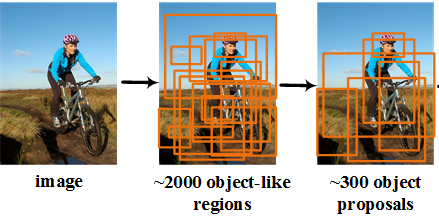
\includegraphics[height=4cm,keepaspectratio=true,clip=true]{imagenes/Logos/regionProposal.png}
  \caption{Ejemplo del método regiones propuesta \\ (Adaptado de:{http://www.cs.toronto.edu/~byang/})}
	\label{Fig: propsalregion}
\end{figure}

Existen dos enfoques emergentes en la actualidad para generar \textit{Regiones Propuestas} \citep{proposal}:
\begin{enumerate}
\item \textbf{Métodos por agrupamiento}: genera múltiples segmentos que puedan corresponder al objeto.
	\begin{itemize}
	\item Selective Search
    \item RandomizedPrim
    \item Ratalankila
    \item Chang
    \item CPMC
    \item Endres
    \item Rigor
    \item Geodesic
	\end{itemize}
\item \textbf{Métodos por puntuación}: estos métodos toman la puntuación (score) de cada candidato según la probabilidad que contenga un objeto de interés.
    \begin{itemize}
    \item Objectness
    \item Rahtu
    \item BING
    \item Edge Boxes
    \item Feng
    \item Zhang
    \item RandomizedSeeds
    \end{itemize}
\item \textbf{Métodos alternativos}: 
    \begin{itemize}
    \item ShapeSharing
    \item Multibox
    \end{itemize}
\end{enumerate}

\subsubsection{Edges Boxes} \label{sub:edgesboxes}

Edges Boxes es un enfoque para la generación de regiones candidatas a partir de los bordes detectados. Utilizando estructuras de datos eficientes, se pueden evaluar millones de boxes (cajas) candidatos en una fracción de segundo; los bordes proporcionan una representación simplificada pero informativa de una imagen \citep{edges}.

Los algoritmos para la detección de bordes tradicionales utilizan una variedad de métodos para calcular gradientes de color, en el caso de los nuevos enfoques además utilizan múltiples características como entrada; incluyendo brillo, color, textura y  escalas de la imagen. 

En la figura (\ref{Fig: edges}) podemos ver de manera simplificada los pasos del método;  en la parte inferior de la imagen vemos que luego de varios operaciones identifica regiones que podrían ser de interés.

\begin{figure}[H]
 \centering
  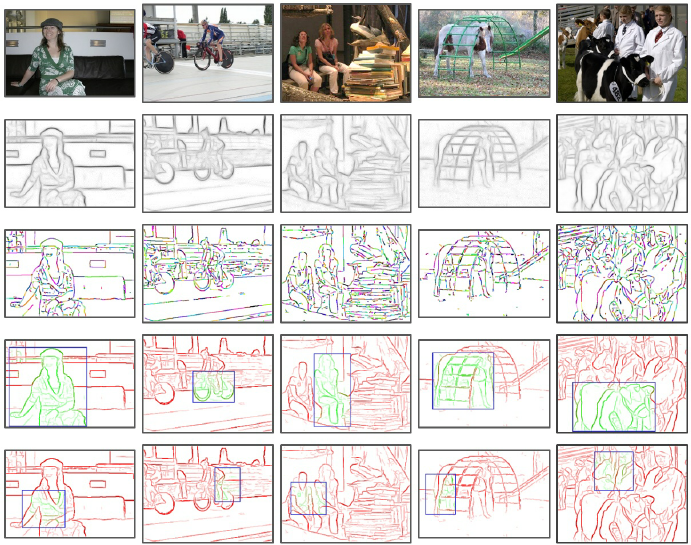
\includegraphics[height=7cm,keepaspectratio=true,clip=true]{imagenes/Logos/edges.png}
  \caption{Ejemplo proceso detección de bordes (Adaptado de:\citep{edges})}
	\label{Fig: edges}
\end{figure}

Este método evalúa las cajas candidatas utilizando un enfoque de ventana deslizante, similar a la detección de objetos tradicionales; donde en cada posición del objeto evaluamos, escala y relación generando una puntuación (score) que indica la probabilidad de que un objeto esté presente.

\subsubsection{BING} \label{sub:bing}
\ac{bing}, puede ser usado para una eficiente estimación de objetos; es un método que propone reducir la ventana de detección a 8x8 y usar la norma de gradiente\footnote{Fuente :https://es.wikipedia.org/wiki/Gradiente} como  un simple vector de 64 dimensiones, realizando una binarización  de estas características.

\ac{bing}  es un modelo lineal, donde:  \(w \in R^{64} \)  y pude ser aproximado por un conjunto de vectores bases. La clave esta en como binarizar y calcular la norma de gradiente eficientemente. Aproximamos la norma de gradiente, cada una tiene un BYTE de valor, usando los bits de parte superior de los valores del BYTE (ver Fig: \ref{Fig: bing}).
\begin{figure}[H]
 \centering
  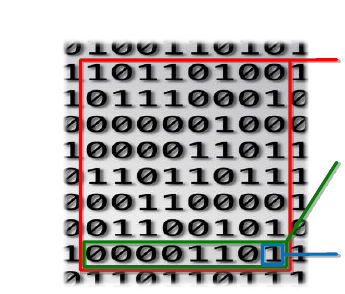
\includegraphics[height=6cm,keepaspectratio=true,clip=true]{imagenes/Logos/BING.png}
  \caption{Ejemplo \ac{bing}. (Adaptado de:\citep{bing})}
	\label{Fig: bing}
\end{figure}


\begin{figure}[H]
 \centering
  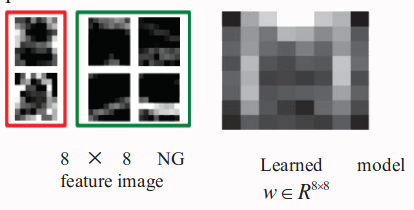
\includegraphics[height=7cm,keepaspectratio=true,clip=true]{imagenes/Logos/bing2.png}
  \caption{Ejemplo de la norma de gradiente de una ventana y el modelo aprendido.(Adaptado de:\citep{bing2})}
	\label{Fig: bing2}
\end{figure}


\subsubsection{Selective Search} \label{sub:selectivesearch}
Selective Search es un método de \textit{Regiones Propuestas} que  permite obtener regiones candidatas realizando una búsqueda exhaustiva aplicando segmentación sobre la imagen. La segmentación  en procesamiento de imágenes consiste en dividirla en grupo de píxeles u objeto. El objetivo es simplificar la representación logrando que sea mas significativa, fácil de analizar y capturar todas las ubicaciones de objetos posibles; en lugar de una sola técnica para generar ubicaciones , diversifica la  búsqueda y usa  una variedad de particiones de imágenes complementarias para tratar con tantas condiciones de imagen como sea posible \citep{selectivesearch}.
Las estrategias usadas en este método son:
\begin{itemize}
\item \textbf{Capturar todas las escalas}: los objetos pueden estar en cualquier escala de la imagen, es por esto que se toma en cuenta todas las escalas.
\item \textbf{Diversificación}: No existe una sola estrategia sino que una región puede formar un objeto solo por color o textura.
\item \textbf{Rápido computo}: Esta es una de las estrategias principales debido a que el objetivo es producir un conjunto de regiones propuesta de manera eficiente y sin un costo computacional alto.
\end{itemize}

\begin{figure}[h]
 \centering
  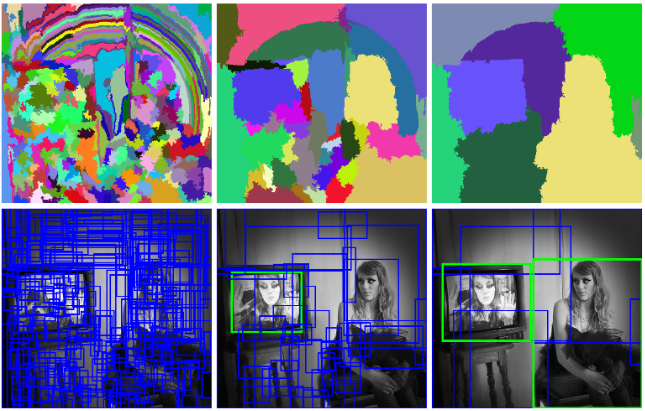
\includegraphics[height=7cm,keepaspectratio=true,clip=true]{imagenes/Logos/selectivesearch.png}
  \caption{Ejemplo segmentación con \textit{Selective Search} (Adaptado de:\citep{selectivesearch})}
	\label{Fig: overlapping}
\end{figure}


\subsection{Non-Maximum Suppression (NMS)}\label{sub:nonmaximumsuppression}

\ac{nms} es un pre-procesamiento muy importante en el ámbito de \ac{va}  donde trabajamos con imágenes de alta resolución \citep{nms}.  \ac{nms} normalmente se usa con algoritmos de detección de bordes \textit{Edge Boxes} .

Puede  suceder que cuando aplicamos métodos de regiones propuestas existan boxes (regiones) con sobremuestreo, es decir lo que en la literatura se los llama \textit{overlapping bounding boxes} , como por ejemplo ver en la figura (\ref{Fig: overlapping}). 

\begin{figure}[H]
 \centering
  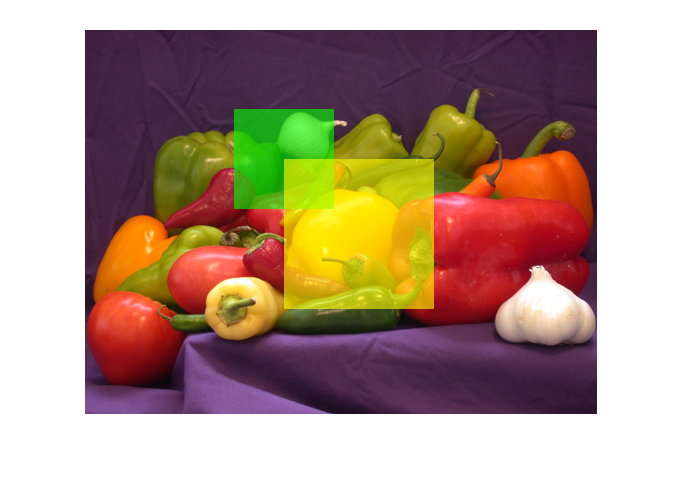
\includegraphics[height=7cm,keepaspectratio=true,clip=true]{imagenes/Logos/overlapMat.png}
  \caption{Overlapping entre regiones (Adaptado de:{https://goo.gl/ihYMvX})}
	\label{Fig: overlapping}
\end{figure}

Para poder eliminar este solapamiento (detecciones redundantes) utilizamos \ac{nms}. \ac{nms} puede ser formulado como una búsqueda de los máximo locales, donde el máximo local es  mayor que todos sus vecinos (\ref{Fig: interseccion}). El algoritmo selecciona aquellas detecciones con un \textit{score} (intersección) alto y elimina los vecinos mas cercanos ya que es muy probable que cubran el mismo objeto \citep{nms2}.

\begin{figure}[h]
 \centering
  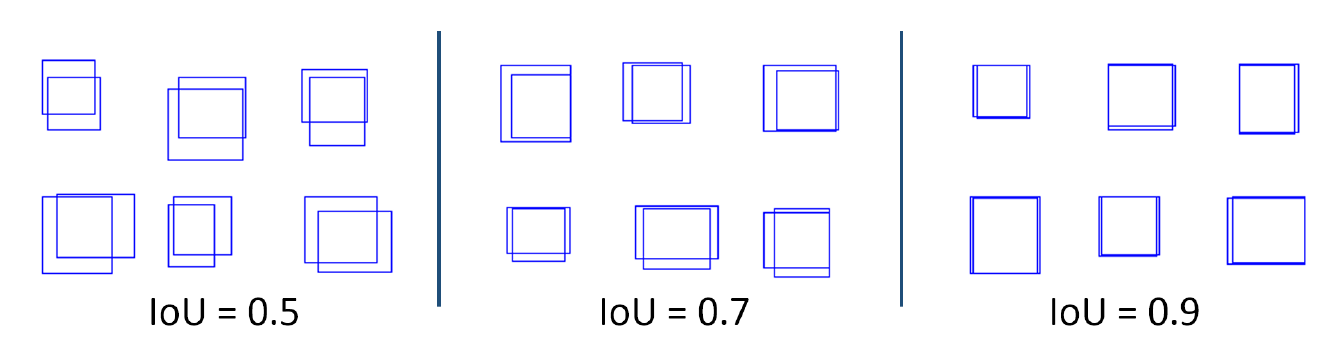
\includegraphics[height=4cm,keepaspectratio=true,clip=true]{imagenes/Logos/overlapping.png}
  \caption{Ejemplo de Overlapping con diferentes scores. (Adaptado de:\citep{edges})}
	\label{Fig: interseccion}
\end{figure}
Dependiendo del valor de score usado podremos eliminar las detecciones redundantes y lograr una mayor optimización  en el reconocimiento. Para obtener una visión mas general del método podemos ver la siguiente figura \ref{Fig: nonmaximumsuppression}.



\begin{figure}[H]
 \centering
  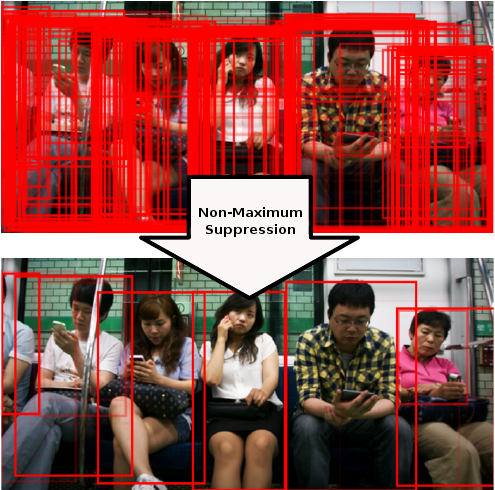
\includegraphics[height=8cm,keepaspectratio=true,clip=true]{imagenes/Logos/nms.png}
  \caption{Uso de non-maximum suppression. (Adaptado de:\citep{nms2})}
	\label{Fig: nonmaximumsuppression}
\end{figure}

En \ac{va} este método es muy utilizado ya que nos permite además de eliminar detecciones redundantes, ayuda a mejorar la clasificación de la imagen optimizando también el tiempo de procesamiento en la clasificación.



\section{Redes Neuronales}\label{sec:redesneuronales}

Las \ac{nn} han sido empleadas satisfactoriamente para problemas de \ac{va}. Estas \ac{nn} son sistemas de redes interconectadas. Existen diferentes tipos de \ac{nn} que resuelven diferentes problemas en el área de \ac{va}. La teoría y representación de los distintos tipos de redes está motivada por la funcionalidad y representación de las redes neuronales biológicas \citep{bernd}. Una \ac{nn} es un modelo matemático que simula el comportamiento de las neuronas del celebro.

En el siguiente diagrama vemos una arquitectura simplificada de una red neuronal (ver:\ref{Fig: redneuronal}).
\begin{figure}[H]
 \centering
  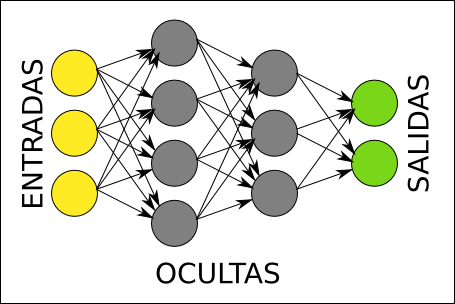
\includegraphics[height=5cm,keepaspectratio=true,clip=true]{imagenes/Logos/neural-net1.png}
  \caption{Red Neuronal \\(Adaptado de:{https://goo.gl/cWaInm})}
	\label{Fig: redneuronal}
\end{figure}

Las \ac{nn} se organizan en capas de la cual cada capa es una neurona, las capas inferiores, ocultas, son las que realiza las operaciones matemáticas correspondiente.  

Debido a su constitución y a sus fundamentos, las redes neuronales artificiales presentan un gran número de características semejantes a las del cerebro. Por ejemplo, son capaces de aprender de la experiencia, de generalizar de casos anteriores a nuevos casos, de abstraer características esenciales a partir de entradas que representan información irrelevante, etc. Esto hace que ofrezcan numerosas ventajas y que este tipo de tecnología se esté aplicando en múltiples áreas. Entre las ventajas se incluyen:
\begin{itemize}
\item \textit{Aprendizaje Adaptativo}. Capacidad de aprender a realizar tareas basadas en un entrenamiento o en una experiencia inicial.
\item \textit{Auto-organización}. Una red neuronal puede crear su propia organización o representación de la información que recibe mediante una etapa de aprendizaje.
\item \textit{Tolerancia a fallos}. La destrucción parcial de una red conduce a una degradación de su estructura; sin embargo, algunas capacidades de la red se pueden retener, incluso sufriendo un gran daño.
\item \textit{Operación en tiempo real}. Los cómputos neuronales pueden ser realizados en paralelo; para esto se diseñan y fabrican máquinas con hardware especial para obtener esta capacidad.
\item \textit{Fácil inserción dentro de la tecnología existente}. Se pueden obtener chips especializados para redes neuronales que mejoran su capacidad en ciertas tareas. Ello facilitará la integración modular en los sistemas existentes
\end{itemize}

Una neurona recibe diversas entradas por medio de interconexiones y retorna una salida, este retorno se da a través de tres funciones característica:
\begin{itemize}
\item Función de propagación: calcula la combinación de cada entrada modificada por el peso de su interconexión. Normalmente se usa como la suma ponderada de las entradas multiplicadas por los pesos.
\item Función de Activación: recibe como entrada a la función de propagación , aunque puede o no utilizarse; existen diversas funciones de activación, tales son los ejemplos de Función Sigmoide, Tangente Sigmoide, Escalón, Lineal, Gaussiana, entre otras.
\item Función de transferencia o  de salida: aplicada al valor devuelto por la función de activación.
\end{itemize}
La siguiente figura (ver: \ref{Fig: redneuronal2}), nos muestra una arquitectura simplificada de una red neuronal aplicada al reconocimiento de patrones.

\begin{figure}[H]
 \centering
  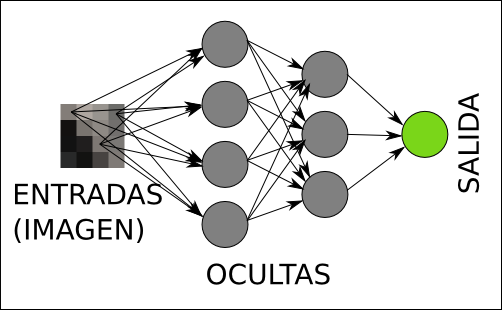
\includegraphics[height=5cm,keepaspectratio=true,clip=true]{imagenes/Logos/neural-net-sample1.png}
  \caption{Ejemplo de red neuronal  \\(Adaptado de:{https://goo.gl/cWaInm})}
	\label{Fig: redneuronal2}
\end{figure}
Estos modelos son  muy flexibles, pudiéndose variar el tipo de neurona en cada capa y su forma de interconexión adaptando a un objetivo particular.

\subsubsection{Redes Neuronales Convolucionales - CNN}

\ac{cnn} son una clase de redes neuronales muy utilizadas en la actualidad por profesionales en \ac{va}. La arquitectura de una \ac{cnn} consiste en múltiples capas donde cada una de estas tienen diferente propósito.

\begin{figure}[h]
 \centering
  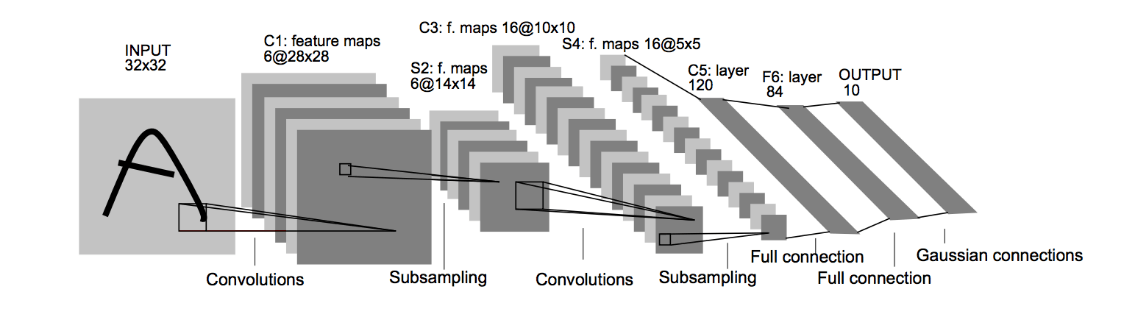
\includegraphics[height=5cm,keepaspectratio=true,clip=true]{imagenes/Logos/cnnconv.png}
  \caption{Red Neuronal Convolucional (Adaptado de:\citep{cnns})}
	\label{Fig: redconvolucion}
\end{figure}

Las \ac{cnn} trabajan modelando de forma consecutiva pequeñas piezas de información (sub-regiones) de la imagen; combinando esta información de salida en las capas mas profundas (ver: \ref{Fig: redconvolucion}), tales características pude ser fusionada pre-procesandolas con el fin de detectar características de mayor orden \citep{murphy}.


El conjunto de salidas de las neuronas en un plano se denomina \textit{mapa de características} (ver \ref{Fig: fmaps}). Cada unidad  del mapa de característica es lo que llamamos en la sección (\ref{sub:problemadeteccion}),  \textit{\textbf{feature vector}}. Una capa convolucional completa está compuesta de varios mapas de características (con diferentes 
\textit{feature vector}), de modo que se pueden extraer múltiples características en cada ubicación \citep{cnns}.

\begin{figure}[H]
 \centering
  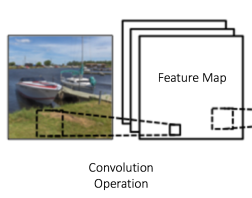
\includegraphics[height=6cm,keepaspectratio=true,clip=true]{imagenes/Logos/fmaps.png}
  \caption{Ejemplo de mapa de caracteristicas, (Adaptado de: \citep{cnnsarticle})}
	\label{Fig: fmaps}
\end{figure}

El tamaño del mapa de características se controla mediante tres parámetros \citep{cnnsarticle}:
\begin{enumerate}
\item depth (profundidad): corresponde al numero de filtros usados para la operación de convolución. Por ejemplo la primera capa toma la imagen original, luego diferentes neuronas a partir de la profundidad de la red se activa realizando operaciones como puede ser retección de bordes, color, etc
es decir a partir de la imagen de entrada aplicar por ejemplo detección de bordes, color, etc.
\item stride (paso): es el número de píxeles por los que se desliza nuestra matriz de filtro sobre la matriz de entrada. Tener un stride grande producirá mapas de características más pequeños.
\item zero-padding (cero-relleno): A menudo, es conveniente rellenar la matriz de entrada con ceros alrededor del borde, de modo que podamos aplicar el filtro a los elementos fronterizos de nuestra matriz de imagen de entrada. Una buena característica de cero relleno es que nos permite controlar el tamaño de los mapas de características.
\end{enumerate}



\section{Aprendizaje Automático}\label{sec:aprendizajeautomatico}
El aprendizaje automático, del ingles \textit{Machine Learning} (\ac{ml}), es  una rama de \ac{ia}; que tiene como objetivo desarrollar técnicas que permitan a las computadoras aprender. 

Arthur Samuel, pionero en esta disciplina, definió a \ac{ml} como:
\begin{quote}\centering
 Campo de estudio que da a las computadoras la habilidad para aprender sin ser explicita-mente programado.[Arthur Samuel.1959]
 % definicion "Field of study that gives computers the ability to learn without being explicitly programmed".
\end{quote}

Otras de las definiciones que encontramos en la literatura se define a \ac{ml} como un conjunto de métodos que pueden detectar automáticamente patrones en los datos y luego usar los patrones descubiertos para predecir los datos futuros o para realizar otros tipos de toma de decisiones bajo incertidumbre \citep{murphy}.

En los recientes años muchas aplicaciones han sido desarrolladas, variando desde minería de datos para aprender a detectar transacciones fraudulentas en tarjetas de crédito o para vehículos autónomos aprendiendo a manejar en la vía publica \citep{Mitchell}.

Algunas ramas de la industria y la ciencia que hacen uso de \ac{ml}:

\begin{itemize}
    \item \textbf{Sistemas de Recuperación de Información}: esto hace referencia a buscadores de Internet utilizan técnicas de ML para mejorar la performance de sus búsquedas.
    \item\textbf{ Diagnóstico Médico}: Se utilizan técnicas de ML para asistir a médicos en el diagnóstico según la historia clínica y los síntomas que presenta el paciente.
    \item \textbf{Ciencias biológicas}: Para la clasificación de especies, reconocimiento de tumores o arritmias o patrones en cadenas de ADN. 
    \item \textbf{Finanzas e Industria bancaria}: Para modelos de fraude de consumo de tarjetas de crédito y de predicción de comportamiento en el mercado de valores.
    \item \textbf{Análisis de imágenes}: Para reconocer escritura manuscrita, también otro tipo de objetos dentro de una imagen, como personas, rostros, monumentos arquitectónicos 
o accidentes geográficos, etc.
     \item \textbf{Juegos}: Ya existen muchos juegos, como el Backgammon y las Damas, predecir jugadas o responder a determinados movimiento del oponente.
     \item \textbf{Robótica}: Se utilizan modelos de ML para regular el desplazamiento de robots, planificación de tareas entre otras funciones.	
\end{itemize}


En general un problema de \ac{ml} se considera un conjunto de \textbf{n} ejemplos de datos y a partir de estos datos se intenta predecir las propiedades de los datos desconocidos. 
Podemos separar a \ac{ml} en dos grandes categorías:
\begin{itemize}
	\item \textbf{Aprendizaje supervisado:} Aquellas aplicaciones en las que existen datos u atributos adicionales de los que queremos predecir. Los problemas de aprendizaje supervisado se clasifican en: 
    \begin{itemize}
    	\item  \textbf{Clasificación:} En un problema de clasificación, estamos tratando de predecir los resultados en una salida discreta. En otras palabras, estamos tratando de asignar variables de entrada en categorías discretas . Un ejemplo de problema de clasificación sería el ejemplo de reconocimiento de dígitos manuscritos, en el que el objetivo es asignar cada vector de entrada a uno de un número finito de categorías discretas.
   		\item \textbf{Regresión:} En un problema de regresión estamos tratando de predecir un resultado dentro de una salida continua. Un ejemplo de problema de regresión sería la predicción del rendimiento en un proceso de fabricación química en el que los insumos consisten en las concentraciones de reactivos, la temperatura y la presión.
    \end{itemize}
    \item \textbf{Aprendizaje no supervisado:} El aprendizaje no supervisado nos permite abordar los problemas con poca o ninguna idea de cómo deben ser nuestros resultados. Podemos derivar la estructura de los datos donde no necesariamente conocemos el efecto de las variables. Podemos derivar esta estructura agrupando los datos basados en relaciones entre las variables en los datos. Con el aprendizaje no supervisado no hay una retroalimentación basada en los resultados de la predicción.
    El objetivo de problemas de aprendizaje no supervisados puede ser descubrir grupos de ejemplos similares dentro de los datos, donde se denomina agrupación (clustering), o determinar la distribución de datos dentro del espacio de entrada, conocida como estimación de densidad (density estimation), o proyectar los datos desde un espacio de nivel dimensional alto hasta dos o tres dimensiones con propósitos de visualización \citep{bishop}.
\end{itemize}

\subsection{Aprendizaje supervisado}\label{sub:aprendizajesupervisado}

En la sección anterior hablamos de las diferentes categorías que existen en \ac{ml}, en esta sección explicaremos mas precisamente el problema de la clasificación supervisada. El objetivo de la clasificación es tomar un vector \textit{\textbf{x}} de entrada, llamado vector de característica,y asignarle una de las clases discretas \textit{K} \citep{bishop}.

\begin{equation}
\begin{array}{cc}
x^i = \text{ vector de característica} &  \text{Donde } i \in \mathsf{R} \\
y \in {1,..,K} & \text{con K como numero de clases}
\end{array}
\end{equation}
El escenario mas común, las clases toman valores  disjuntos, donde para cada vector de característica de entrada se le asigna solo a una clase. El espacio de entrada se divide así en regiones de decisión cuyos límites se llaman límites de decisión o superficies de decisión \citep{bishop}.

Si K = 2 se llama clasificación binaria; es decir que en este caso \textit{y} asume valores de (0,1) ; en caso contrario si K > 2, se la llama clasificación multiclase.

Una manera de  formalizar el problema de la clasificación es una función de aproximación también llamada \textbf{función discriminante}, en donde: \textit{y = f(x)} para alguna función \textit{f} ; el objetivo del aprendizaje es estimar la función \textit{f} dado un conjunto de entrenamiento etiquetado y entonces realizar predicciones usando la siguiente función \ref{eq:funciondiscriminante}:
\begin{equation}\label{eq:funciondiscriminante}
\bar{y}= \overline{f(x)}
% y(x) = w^T x + w
\end{equation}
Nuestro principal objetivo es realizar las predicciones sobre vectores de característica nuevos, es decir, aquellos que no hemos entrenado. La clasificación es probablemente la forma más utilizada en algoritmos de aprendizaje automático, y se ha utilizado para resolver muchos problemas interesantes y a menudo difíciles del mundo real  \citep{murphy}.

\begin{figure}[H]
 \centering
  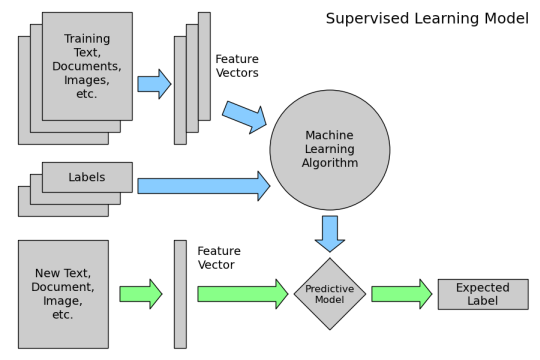
\includegraphics[height=7cm,keepaspectratio=true,clip=true]{imagenes/Logos/01_supervised_learning.png}
  \caption{Modelo de un Sistema de Aprendizaje Supervisado}
	\label{Fig: aprendsupervisado}
\end{figure}

\subsection{Clasificación}\label{sub:clasificacion}
Como se menciono en la sección anterior \ref{sec:aprendizajeautomatico} la clasificación consiste básicamente en asignar un vector de característica a una clase previamente definida.

Los objetos se definen por diversas característica como color, textura o tamaño. Para poder clasificar se debe usar una frontera entre las diferentes clases; estas fronteras se calculan mediante el entrenamiento de las característica del objeto. Clasificar un objeto desconocido es asignar el objeto a una clase, donde las características de este objeto tiene alguna correspondencia con las características de los objetos que se entrenó. 

Independientemente del clasificador que se utilice el proceso de clasificación consta de una serie de pasos:
\begin{enumerate}
\item Se reúnen muestras de objetos de clases conocidas, se eligen un conjunto de vectores de característica apropiado.
\item El conjunto de vectores de características se usa para entrenar el clasificador. 
\item Se calculan las fronteras entre las clases. 
\item Se extraen las mismas características de los objetos desconocidos a clasificar.
\item El clasificador usa las fronteras calculadas durante el entrenamiento para decidir a qué clases pertenecen los nuevos vectores de características de los objetos que queremos reconocer.
\end{enumerate}

En un pipeline de reconocimiento (ver: \ref{sec:pipeline}) de patrones los datos de la imagen se representan en un vector de característica 
\textit{feature vector}; estos datos se representan en un denominado espacio de característica. A partir de los datos representados en el espacio de característica se puede observar si existen conglomerados de datos que puedan separarse; es decir la tarea de un clasificador es separar estos agrupaciones (conglomerados) durante el entrenamiento y asignarle una clase conocida.


Los clasificadores que usan hiperplanos para separar las clases se denominan clasificadores lineales, otros clasificadores construyen superficies arbitrarias que permiten separar agrupaciones de datos muy cercanos e incluso que se solapen; estos se los llaman clasificadores no lineales. 

\begin{figure}[h]
 \centering
  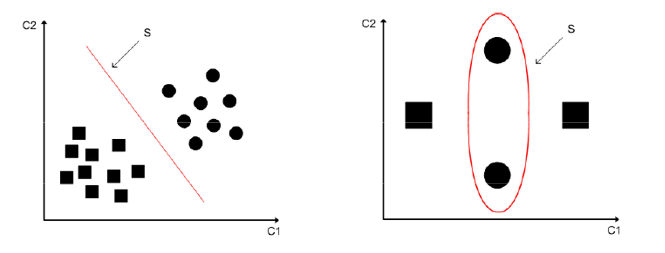
\includegraphics[height=5cm,keepaspectratio=true,clip=true]{imagenes/Logos/clasificador.png}
  \caption{Ejemplo de clasificación lineal (izquierda) y no lineal (derecha) (Adaptado de:{https://goo.gl/VAm6bE})}
	\label{Fig: clasif}
\end{figure}

\subsubsection{Clasificadores SVM}\label{sub:svm}
Las \ac{svm}, son métodos usado para la clasificación. Un clasificador \ac{svm} busca el limite que separa las clases con el mayor margen posible; como podemos ver en la siguiente imagen (\ref{Fig: margenseparacionsvm}).

\begin{figure}[H]
 \centering
  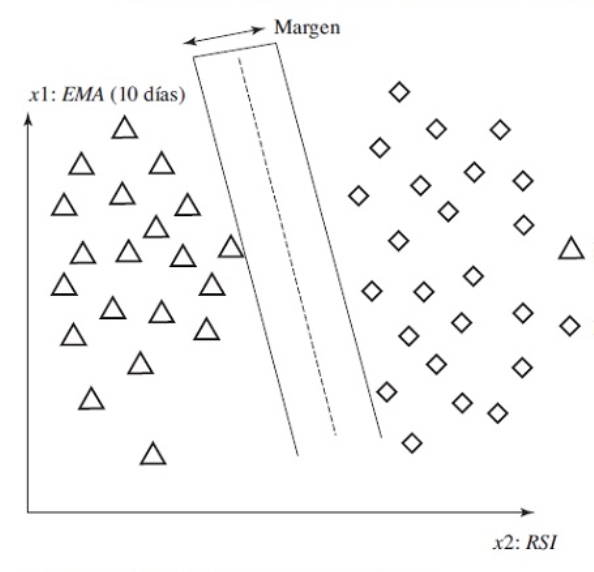
\includegraphics[height=7cm,keepaspectratio=true,clip=true]{imagenes/Logos/separacionsvm.png}
  \caption{Ejemplo margen de Separación hiperplano SVM \\(Adaptado de:{https://goo.gl/eTZfvH})}
	\label{Fig: margenseparacionsvm}
\end{figure}

Las ventajas de las máquinas de soporte de vectores son:
\begin{itemize}
\item Eficaz en grandes espacios dimensionales.
\item Sigue siendo efectivo en casos en los que el número de dimensiones es mayor que el número de muestras.
\item Versátil: se pueden especificar diferentes funciones del kernel para la función de decisión.
\item El proceso de entrenamiento es más rápido en comparación con otros clasificadores, sobre todo para conjunto de entrenamientos grandes.
\end{itemize}



\subsection{El problema de la Clasificación}\label{sub:malaclasificacion}
En \ac{ml} describimos el aprendizaje a partir de los datos de entrenamiento. El objetivo es crear un modelo que generalice el problema a partir de los datos de entrenamiento para poder hacer predicciones de datos desconocidos. Las terminologías utilizadas en \ac{ml} sobre un modelo cuando aprende y generaliza los datos se conoce como  \textit{\textbf{overfitting}} y \textit{\textbf{underfitting}}.

\textit{\textbf{Overfitting}} y \textit{\textbf{underfitting}} son dos grandes problemas en \ac{ml} que influye en la performance del modelo. 

\subsubsection{Overfitting}
Este concepto en \ac{ml} hace referencia al sobreentrenamiento del modelo. El overfitting ocurre cuando un modelo aprende el detalle junto a el ruido en los datos de entrenamiento afectando negativamente el rendimiento del modelo en los nuevos datos a predecir. Esto significa que el ruido o las fluctuaciones aleatorias en los datos de entrenamiento son aprendidos como conceptos por el modelo. El problema es que estos conceptos no se aplican a los nuevos datos e impactan negativamente en la capacidad de generalización de los modelos.

\subsubsection{Underfitting}
Como parte opuesta al overfitting esta el  underfitting; este concepto hace referencia a aquellos modelos que no pueden generalizar nuevos datos de entrenamiento de manera correcta. Mayormente en problemas de underfitting se necesita mayores caracteristicas de los datos para la construcción de los modelos.

\begin{figure}[h]
 \centering
  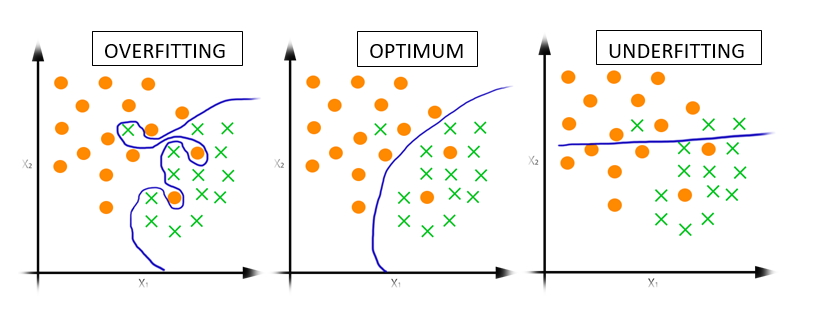
\includegraphics[height=5cm,keepaspectratio=true,clip=true]{imagenes/Logos/OverFUnderF.png}
  \caption{Ejemplo de overfitting (izquierda), modelo óptimo (centro) y underfitting (derecha)}
	\label{Fig: overUnder}
\end{figure}

Una de las técnicas para evitar problemas en la creación de modelos predictivos es por medio de un conjunto de validación. Como veremos a continuación a través de técnicas de \textit{cross-validation} podemos evaluar los modelos y obtener una idea de como este modelo puede generalizar los datos de manera correcta.

\subsection{Técnicas de Validación}\label{sub:tecnicasvalidacion}
Existen diversas técnicas sobre validación en la literatura de \ac{ml}; una de las mas usada por los profesionales del esta área es, \textit{cross validation} (validación cruzada). La validación cruzada es una técnica que evalúa los resultados de un análisis estadístico y garantiza de que sean independientes de la partición de los datos de entrenamiento y prueba. 

Hay diversos tipos de validación cruzada, la mas utilizada es k-iteraciones o K-Folds; la cual consiste en dividir el conjunto de datos en \textit{k} subconjuntos. El método empleado por esta técnica es dejar uno de los subconjuntos de datos como validación y el resto de entrenamiento, es decir los (\textit{k}-1) subconjuntos. Este proceso se repite durante \textit{k} iteraciones con cada uno de los subconjunto de dato de validación. Para finalizar se utilizar aquel subconjunto de datos que posea mayor generalidad.

En el siguiente diagrama (ver:\ref{Fig: crossvalidation})se muestra de manera mas intuitiva el proceso llevado a cabo por esta técnica.

\begin{figure}[H]
 \centering
  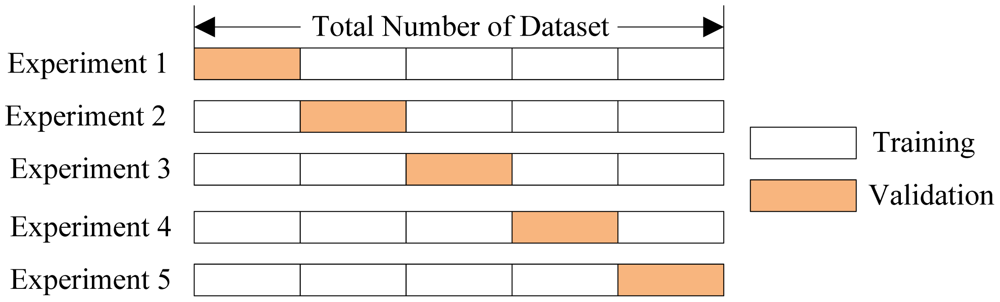
\includegraphics[height=5cm,keepaspectratio=true,clip=true]{imagenes/Logos/crossvalidat.png}
  \caption{Validación cruzada para k=5\\(Adaptado de:{http: //goo.gl/Dp85h3})}
	\label{Fig: crossvalidation}
\end{figure}

\section{Pipeline}\label{sec:pipeline}
Hablar de pipeline en el ámbito de \ac{ml}, se refiere al flujo de trabajo u etapas del proyecto que pueda ser automatizado; esto proporciona una abstracción de alto nivel del flujo de aprendizaje y simplifican en gran medida el flujo de trabajo completo.

Un pipeline clásico que se usa en el desarrollo de proyectos en \ac{ml} es el que se muestra a continuación:
\begin{figure}[H]
 \centering
  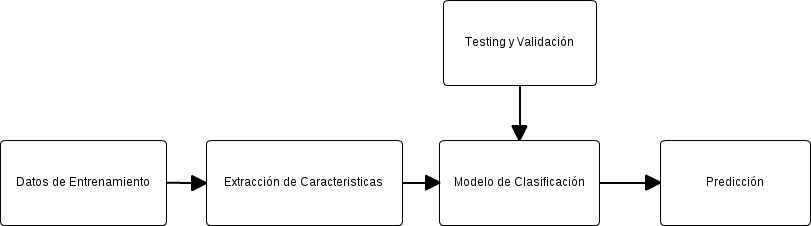
\includegraphics[height=3cm,keepaspectratio=true,clip=true]{imagenes/Logos/pipelineclasico.png}
  \caption{Pipeline Clásico de \ac{ml}}
	\label{Fig: pipelineclasico}
\end{figure}

Partiendo del modelo clásico anterior, adaptamos el pipeline de acuerdo a las necesidades del proyecto, esto se visualiza en la siguiente figura (\ref{Fig: pipeline}):

\begin{figure}[H]
 \centering
  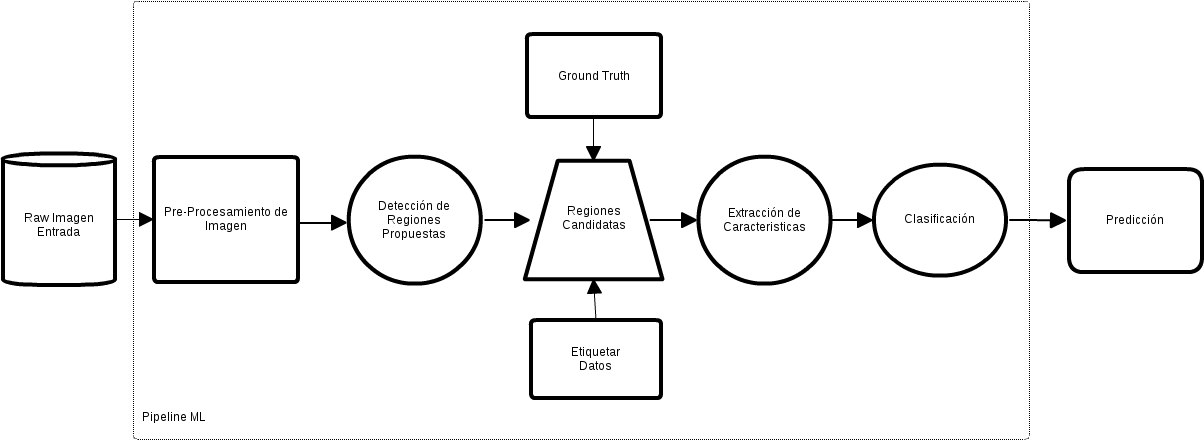
\includegraphics[height=6cm,keepaspectratio=true,clip=true]{imagenes/Logos/pipeline.png}
  \caption{Pipeline}
	\label{Fig: pipeline}
\end{figure}

